% Noah
\section{Markenanalyse} \label{sec:markenanalyse}

\subsection{Branding}
Garmin ist bekannt für seine Sportuhren, die eine klare visuelle Identität aufweisen. Ein charakteristisches Merkmal ist das Logo von Garmin selbst, das in der Regel auf den Uhren präsent ist. Das Logo besteht aus einer stilisierten schwarzen Schrift auf einem weißen Hintergrund, was eine gewisse Seriosität und Zuverlässigkeit vermittelt. Das blaue Dreieck steht für Erfolg, Wachstum und Entwicklung wobei der Blauton Zuverlässigkeit und Stabilität demonstriert. \cite{logo}

\begin{figure}[H]
    \centering
    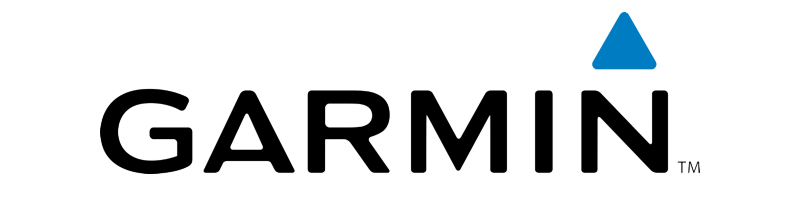
\includegraphics[width=0.6\linewidth]{Figure/logo.png}
    \caption{Garmin Logo \cite{logo}}
    \label{fig:logo}
\end{figure}

Diese Farbkombination ist einprägsam und sofort mit der Marke verbunden. Zusätzlich sind die Uhren oft in sportlichen Farben wie Schwarz, Rot, oder Blau erhältlich, die Dynamik und Energie ausstrahlen. Symbole und Formen auf den Uhren sind oft funktional, wie zum Beispiel klare Ziffernblätter, intuitive Bedienungsknöpfe und auch grafische Elemente, die Aktivitäten repräsentieren. Diese visuellen Ausdrucksformen tragen dazu bei, dass Garmin-Uhren nicht nur als Sportausrüstung, sondern auch als Modeaccessoire wahrgenommen werden.

\subsection{Markenarchitektur}\label{Markenarchitektur}
Garmin verfolgt im Allgemeinen eine 'Branded House' Strategie, wobei die Hauptmarke Garmin als 'Dachmarke' fungiert und verschiedene Produkte (meist mit Zusammenhang) unter einem Namen anbietet. In diesem Fall umfasst dies nicht nur Sportuhren, sondern auch andere GPS-Produkte wie Navigationsgeräte, Wearables und Outdoor-Geräte. Alle diese Produkte tragen das Garmin-Logo und profitieren von der starken Markenbekanntheit und Reputation, die Garmin aufgebaut hat. Durch diese konsistente Markenführung schafft Garmin Vertrauen bei den Verbrauchern und ermöglicht es ihnen, verschiedene Produkte der Marke mit derselben Qualität und Zuverlässigkeit zu verbinden.
